\usetikzlibrary{calc}


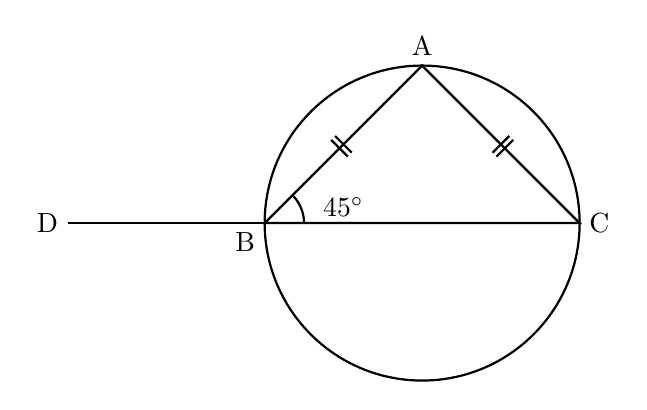
\begin{tikzpicture}[scale=1]
    % Define radius of the circle
    \def\R{2}

    % Define center of the circle
    \coordinate (O) at (0,0);

    % Define points B and C on the circle such that BC is a diameter
    \coordinate (B) at (-\R,0);
    \coordinate (C) at (\R,0);

    % Draw the circle
    \draw[thick] (O) circle (\R);

    % Define point A on the circle
    % Angle is chosen to make AB and AC approximately equal length as visually indicated
    \coordinate (A) at (90:\R);

    % Draw lines AB, AC, BC
    \draw[thick] (B) -- (A) -- (C) -- cycle;
    \draw[thick] (B) -- (C); % Redraw BC to ensure it's on top if needed

    % Define point D on the extended line CB
    \coordinate (D) at (-4.5,0); % Extending to the left

    % Draw the extended line segment DB
    \draw[thick] (D) -- (B);

    % Draw the angle arc at B (angle ABC)
    \draw[thick] (B) +(0:0.5) arc (0:45:0.5);

    % Add the angle label
    % Shifted the x-coordinate from -1.3 to -1.0 to move it to the right
    \node at (-1.0, 0.2) {$45^\circ$};

    % Add the equality tick marks on AB and AC
    % Calculate midpoints and angles for proper tick placement
    \coordinate (midAB) at ($(A)!0.5!(B)$);
    \coordinate (midAC) at ($(A)!0.5!(C)$);

    % Angle of AB is roughly 45 degrees, so perpendicular is 135 / -45
    \draw[thick] ($(midAB) + (-45:0.15)$) -- ($(midAB) + (135:0.15)$);
    \draw[thick] ($(midAB) + (-0.05,-0.05) + (-45:0.15)$) -- ($(midAB) + (-0.05,-0.05) + (135:0.15)$);

    % Angle of AC is roughly -45 degrees (from horizontal left), so perpendicular is 45 / 225
    \draw[thick] ($(midAC) + (45:0.15)$) -- ($(midAC) + (225:0.15)$);
    \draw[thick] ($(midAC) + (0.05,-0.05) + (45:0.15)$) -- ($(midAC) + (0.05,-0.05) + (225:0.15)$);

    % Add labels for the points
    \node[above] at (A) {A};
    \node[below left] at (B) {B};
    \node[right] at (C) {C};
    \node[left] at (D) {D};

\end{tikzpicture}